% Translate the eight points of x^2+y^2=1 by (0,1); the image is x^2+(y-1)^2=1.
\documentclass[tikz,border=8pt]{standalone}
\usepackage{amsmath,amssymb}
\usetikzlibrary{arrows.meta}
\begin{document}
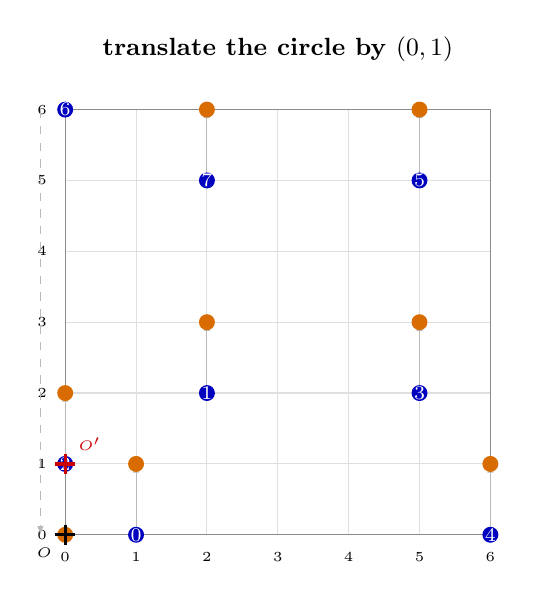
\begin{tikzpicture}[scale=0.9]
  \draw[gray!25] (0,0) grid (6,6);
  \draw[black!45] (0,0) rectangle (6,6);
  \foreach \x in {0,...,6} {%
    \node[font=\tiny,below] at (\x,-0.12) {\x};%
    \node[font=\tiny,left] at (-0.12,\x) {\x};%
  }
  % translation arrows (the wrap is dashed, outside the grid)
  \foreach \x/\y in {1/0,2/2,0/1,5/2,6/0,5/5,2/5} {%
    \draw[gray!55, -{Latex[length=1.1mm]}] (\x,\y)--(\x,\y+1);}
  \draw[gray!55, -{Latex[length=1.1mm]}, dashed] (-0.35,6)--(-0.35,0);
  % original conic points
  \foreach \x/\y/\k in {1/0/0,2/2/1,0/1/2,5/2/3,6/0/4,5/5/5,0/6/6,2/5/7} {%
    \fill[blue!75!black] (\x,\y) circle (3.2pt);%
    \node[font=\scriptsize,text=white] at (\x,\y) {\k};%
  }
  % translated points
  \foreach \x/\y in {1/1,2/3,0/2,5/3,6/1,5/6,0/0,2/6} {%
    \fill[orange!85!black] (\x,\y) circle (3.2pt);%
  }
  % centres: O=(0,0) black, O'=(0,1) red
  \draw[black, very thick] (-0.14,0)--(0.14,0) (0,-0.14)--(0,0.14);
  \draw[red!80!black, very thick] (-0.14,1)--(0.14,1) (0,0.86)--(0,1.14);
  \node[font=\tiny,black,below left] at (-0.05,-0.05) {$O$};
  \node[font=\tiny,red!80!black,above right] at (0.05,1.05) {$O'$};
  \node[font=\small\bfseries] at (3,6.85) {translate the circle by $(0,1)$};
\end{tikzpicture}
\end{document}
